\chapter{Nonlinear Correlations and Measurement-Induced Phase Transitions}
\thispagestyle{empty}
\label{chap:MIPT_continuous_measurement}

In this chapter, we present a project which evolved from the work presented in the previous chapter. We saw that we can model free fermions for larger system sizes, and this makes it natural to explore ways to experimentally detect the measurement-induced phase transition discovered by Alberton et al.~\cite{alberton2021}. We show that a correlation function, which we introduce below, is able to distinguish between the two phases that emerge when changing the measurement strength. Moreover, we are able to reconstruct this correlation function from linear information extracted from many measurement trajectories. This initially suggests that it might be possible to extract the behavior of the correlation function from the noisy measurement record, which emerges naturally from our measurement scheme. However, what can be measured is very subtle, and we found that this cannot be directly measured in experiments. In this chapter, we present the work we did in this project and also show why it is not possible to extract any nonlinear information from different measurement outcomes.

\section{Introduction}

In chapter~\ref{chap:MIPT_bosons}, we explored a system consisting of hardcore bosons where coherent dynamics compete with projective measurements, leading to measurement-induced phase transitions. We simulated the non-interacting case for free fermions as it allowed us to access larger system sizes and helped in our analysis of the bosonic system. In this chapter, however, we will exclusively consider free fermions and explore whether we can detect the transition resulting from the competition between coherent Hamiltonian dynamics and continuous local weak measurement~\cite{szyniszewski2019,romito2020}, illustrated in Fig.~\ref{fig:Chapter4_Fig1}a). In this model, the system undergoes a MIPT from a critical to an area-law regime~\cite{alberton2021}, with a schematic representation of the phase diagram in Fig.~\ref{fig:Chapter4_Fig1}b).

    \begin{figure}[ht]
        \centering
        \includegraphics[width = \textwidth]{Chapters/Plots/Chapter5/Chapter4_Fig1.pdf}
        \caption{a) Schematic representation of free fermions on a 1D chain with nearest-neighbor hoping and subject to continuous measurement of the local particle number. b) Schematic representation of the phase diagram as a function of the measurement strength $\gamma$.}
        \label{fig:Chapter4_Fig1}
    \end{figure}
    
As we saw in chapter~\ref{chap:MIPT_bosons}, these phases are characterized by a logarithmic scaling of the entanglement entropy in the critical regime and constant entanglement entropy with subsystem size in the area-law regime. Furthermore, we will show that we can distinguish between the two phases using a nonlinear correlation function, which decays algebraically in the critical regime and exponentially in the area-law regime. Although both quantities are extremely useful in characterizing and distinguishing different phases, they cannot be measured efficiently in experiments, as this would require reproducing individual stochastic trajectories more than once. As in previous sections, the MIPT is not present at the level of the density operator as the trajectory-averaged density matrix is the trivial infinite temperature state for any non-zero measurement rate \cite{li2018,li2019,bao2020,alberton2021}, from which we cannot extract any useful information. Nonlinear functions of the state, however, capture information on the competition between the coherent Hamiltonian dynamics and the continuous weak measurements. 

Suitable nonlinear functions include the von Neumann entropy (Eq.~\ref{eq:vnE}), which we already used to distinguish different phases in chapter~\ref{chap:MIPT_bosons}. Furthermore, the second moment of the two-point correlation function $C_2(l,m) = \overline{|\langle \hat{a}^\dagger_l \hat{a}_{m} \rangle|^2}$, (where $\hat{a}^\dagger_i,\hat{a}_i$ are fermionic creation and annihilation operators respectively in site $i$ and $\overline{.\phantom{l}.\phantom{l}.}$ denotes trajectory averaging), displays a non-trivial trajectory average, which we present in the next section. Note that $\langle \hat{a}^\dagger_l \hat{a}_{m} \rangle$ is non-hermitian. However, we consider the second moment of the correlation function and we will see that this quantity can also be expressed as the connected-correlation function between the local fermion densities $\hat{n}_l$ and $\hat{n}_{m}$ (with $\hat{n}_i = \hat{a}_i^\dagger \hat{a}_i$). We continue by introducing the model we consider in this chapter, exploring whether it is possible to reconstruct the correlation function using only linear information in the density operator and the difficulties we have encountered when extending this idea to experimental setups.

\section{Free Fermion Chain with Continuous Weak Measurement}

In this chapter, we consider free fermions on a periodic, one-dimensional chain with nearest-neighbor hopping that are subject to continuous measurement of the local particle number, as illustrated in Fig.~\ref{fig:Chapter4_Fig1}a). The quadratic hopping Hamiltonian for a chain consisting of $M$ sites is, 
\begin{equation}
H =-J \sum\limits_{i=1}^{M} ( \hat{a}^{\dagger}_i \hat{a}_{i+1} + \hat{a}_i \hat{a}^{\dagger}_{i+1}),
\end{equation}
where $J$ is the tunneling amplitude, $\hat{a}^{\dagger}_i$,$\hat{a}_i$ are the respective fermionic creation and annihilation operators on site $i$. We also assume periodic boundary conditions to limit finite-size effects seen in our analysis. Coherent dynamics lead to a build-up of entanglement as particles hop between neighboring sites while the continuous measurement of the local fermion densities $\hat{n}_i = \hat{a}_i^\dagger \hat{a}_i$ reduces entanglement. This competition leads to a MIPT from a critical phase to an area-law phase \cite{alberton2021}, as noted above. 

We consider a specific type of continuous weak measurement \cite{wiseman2009,jacobs2006}, namely homodyne detection ~\cite{barchielli1991,gisin1992,wiseman1993}, which we introduced in section~\ref{subsec:hom_detec} and may be realized via dispersive coupling of the fermions to cavity photons~\cite{yang2018} or fluorescence measurements of superconducting qubits~\cite{campagne-ibarcq2016}. Yang et al. propose a scheme where a scanning microscope monitors the quantum dynamics of a system in a cavity QED setup. In this scheme, atoms manifest their presence via resonance shifts in the output field of the cavity, which is mixed with a local oscillator, resulting in a homodyne current containing information about the atomic densities. Campagne-Ibarcq et al. propose a scheme where the fluorescence field of qubits is measured using heterodyne detection, which allows the authors to gain information about the state of the qubits. 

The time evolution of the fermion wavefunction follows the stochastic Schr\"{o}dinger equation (SSE), which we defined in section \ref{subsec:qsd},
\begin{equation}
\label{eq:SSE1}
    \ket{\psi(t+dt} = \Big(1-iH dt + \sum\limits_{i=1}^M\Big[ \sqrt{\gamma} \tilde n_{i,t} dW_{i,t}- \frac{\gamma}{2} \tilde n_{i,t}^2 dt\Big]  \Big) \ket{\psi_t},   
\end{equation}
where $\tilde n_{i,t} = \hat{n}_i - \expectation{\hat{n}_i}_t$ which includes a state dependence, $\gamma$ is the measurement rate, and $dW_{i,t}$ is Wiener increment with mean $0$ and variance $dt$, satisfying the conditions described in Eq.~\ref{eq:noise}.

As we discussed in section~\ref{sec:FGS}, the SSE \ref{eq:SSE1} is quadratic in fermion operators, and the dynamics of the wave function can be simulated efficiently in terms of Fermionic Gaussian States (FGS). In this case, the fermion wave function is completely characterized by the correlation matrix, $D_{ij} = \langle \hat{a}^\dagger_i \hat{a}_j \rangle$. The detailed numerical procedure is outlined in section \ref{sec:FGS}. 

\section{Reconstruction of the correlation function \texorpdfstring{$C_2(l,m)$}{TEXT} using linear information}

As we have already seen, nonlinear functions allow us to gain insight into the different phases. The critical phase is characterized by logarithmic scaling of the entanglement entropy for small measurement rates and algebraic decay of the correlation function $C_2(l,m)$. However, in the strong measurement regime, measurements prevent entanglement and long-range correlations from building up, resulting in area-law entanglement and exponentially decaying correlations. 

\begin{figure}[ht]
    \centering
    \includegraphics[width=\textwidth]{Chapters/Plots/Chapter5/Chapter4_Fig2.pdf}
    \caption{a) The von Neumann entropy of the approximate stationary state as a function of subsystem $M_A$ ($M = 40$) for measurement strengths, $\gamma = 0.1, 0.5, 5, 10$. b) The correlation function $C_2(1,1+l) = |\expectation{a_1^\dagger a_{1+l}}|^2$ as a function of distance $l$. We time-evolve until $TJ = 60$ and compute trajectory averages using $N_t = 10^6$ trajectories. The legend presented in a) applies also to b).}
    \label{fig:Chapter4_Fig2}
\end{figure}

In Fig.~\ref{fig:Chapter4_Fig2}~a), we plot the von Neumann entropy in the approximate steady state as a function of the subsystem size for a range of measurement strengths. We observe logarithmic scaling of the entropy with the subsystem size for the small measurement strengths. In contrast, in the large measurement regime, the entanglement only grows minimally and afterward remains constant. In Fig.~\ref{fig:Chapter4_Fig2}~b), we plot the correlation function $C_2(1,1+l)$ as a function of the distance $l$, which also witnesses the transition. For small measurement strengths, we observe the correlation function follows the same qualitative behavior as that of the curve $(1+l)^{-2}$, indicating algebraic decay. We also observe the characteristic exponential decay of the correlation function with the distance $l$ for the large measurement strengths, which is indicated here by the linear downward trend on the logarithmic scale.

As noted before, we cannot measure these quantities in an experiment as this would require accessing individual trajectories multiple times. We can, however, express the connected correlation function in terms of number operators \cite{alberton2021}, 
\begin{equation}
    C_2(l,m) = \overline{|\langle \hat{a}^\dagger_l \hat{a}_{m} \rangle|^2} = \overline{\expectation{\hat{n}_l} \expectation{\hat{n}_m}} - \overline{\expectation{\hat{n}_l \hat{n}_m}},
\end{equation}
where $\expectation{n_i}$ are the expectation values of the local number operators in site $i$. The second term in this expression $\overline{\expectation{\hat{n}_l \hat{n}_m}}$ corresponds to the linear average in the infinite temperature state and is determined by the initial state. We consider an initial product state at half filling, and as we time-evolve under a number-conserving Hamiltonian, the total particle number does not change. 
Therefore, if we measure $n_m$ the probability of detecting a particle at site $m$ to not detecting it is $N/M$ on average, and then as we have $N-1$ particles left, spread over $M-1$ sites, the probability of detecting a particle at site $l$ to not detecting it, is $\dfrac{N-1}{M-1}$ on average after measuring $n_m$. Hence we have, 
\begin{equation}
    \overline{\expectation{\hat{n}_l \hat{n}_m}} = \frac{N}{M}\frac{N-1}{M-1},
\end{equation}
where $N = M/2$ as we only consider initial states at half-filling. Note that in the thermodynamic limit, as $M\to\infty$, $\overline{\expectation{\hat{n}_l \hat{n}_m}} \to \frac{1}{4}$. Using this we can reconstruct the correlation function $C_2(l,m)$, 
\begin{equation}
   \tilde C_2(l,m) = \overline{\expectation{\hat{n}_l} \expectation{\hat{n}_m}} - \frac{N}{M}\frac{N-1}{M-1},
\end{equation}
where $\tilde C_2(l,m)$ is the correlation function computed directly from the local fermion densities. 

In Fig.~\ref{fig:Chapter4_Fig3}, we plot $\tilde C_2(i,i+l)$ as a function of the distance $l$, where we have averaged over all sites, as well as over the time interval $TJ \in [55, 60]$, to reduce the statistical errors as much as possible. We also plot $C_2(i,i+l)$ to compare it to the reconstructed correlation function.

\begin{figure}[ht]
    \centering
    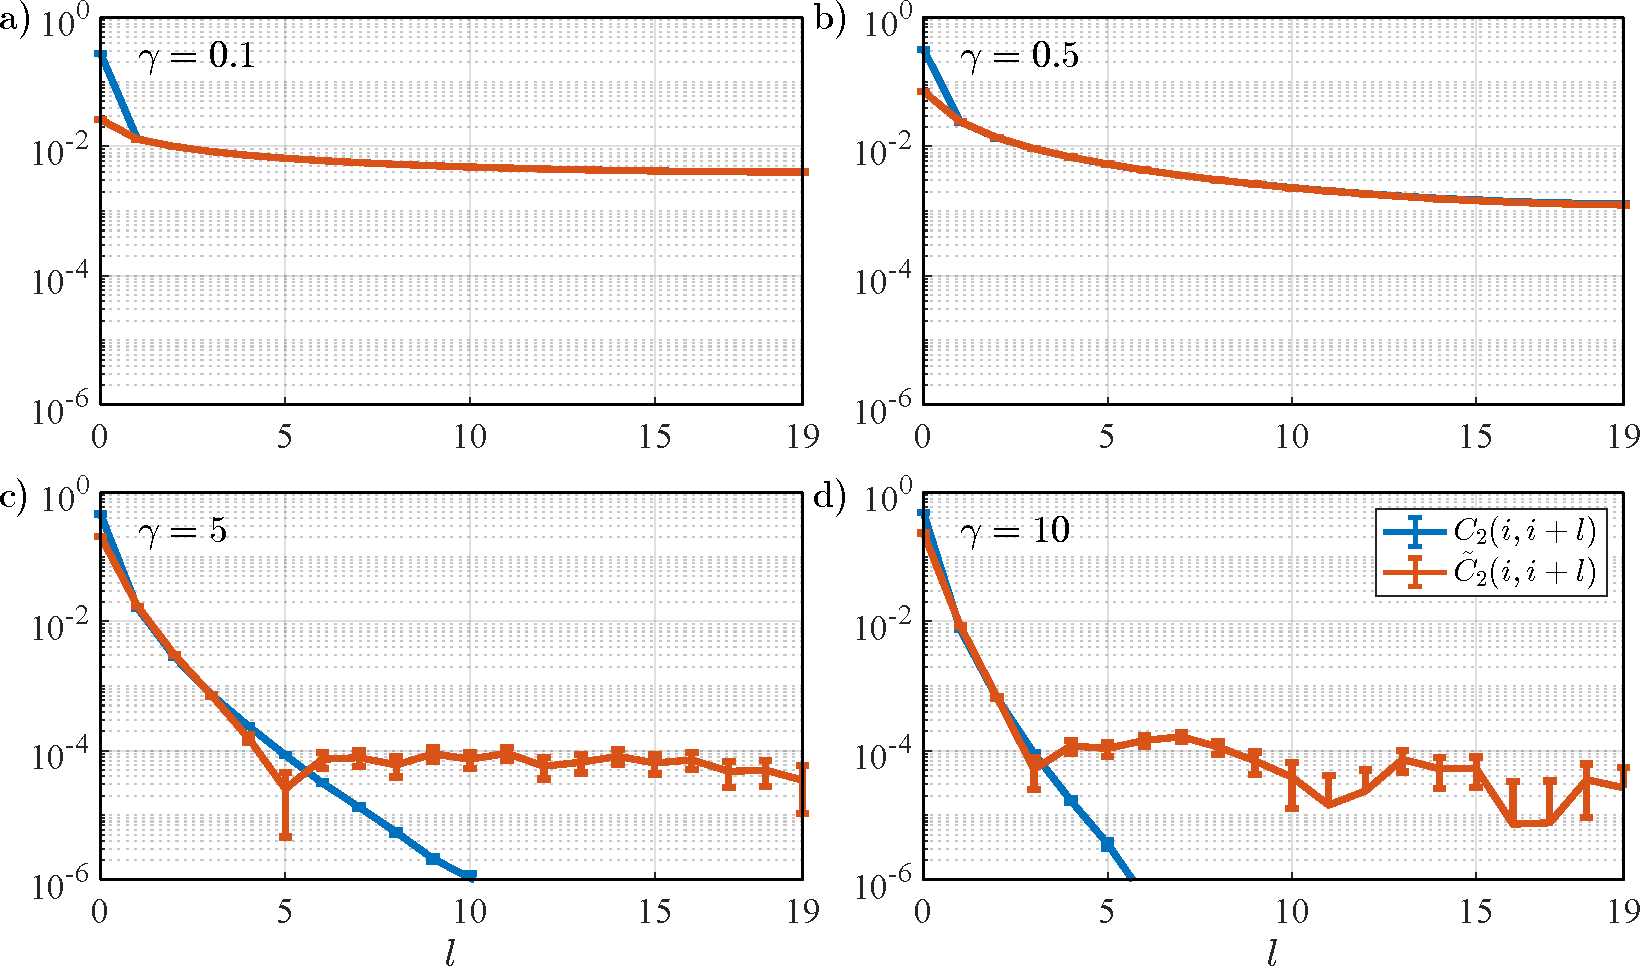
\includegraphics[width=\textwidth]{Chapters/Plots/Chapter5/Chapter4_Fig3.pdf}
    \caption{The second moment of the correlation function $C_2(i,i+l) = |\expectation{a_i^\dagger a_{i+l}}|^2$ as a function of distance $l$. We compare $C_2(i,i+l)$ to $\tilde C_2(i,i+l)$, which is the correlation function computed from the local fermion densities. We time-evolve until $TJ = 60$, with a numerical time step $dt = 0.01$, and compute trajectory averages using $N_t = 10^6$ trajectories. We further average $\tilde C_2(i,i+l)$ over the interval $TJ\in[55,60]$ and spatially average over all sites, $i \in [1,40]$. The legend presented in d) applies also to a)-c).}
    \label{fig:Chapter4_Fig3}
\end{figure}

 In Fig.~\ref{fig:Chapter4_Fig3}~a), b) we plot the correlation functions for $\gamma = 0.1, 0.5$ respectively, and we observe near perfect overlap between the two correlation functions, indicating that this method in the small measurement regime works very well. In the large measurement regime, however, the correlations decay faster than the statistical errors, which we observe in Fig.~\ref{fig:Chapter4_Fig3}~c), d) where we plot the correlation functions for $\gamma = 5, 10$ respectively. We initially see a good agreement to roughly a distance $l \sim 4,5$ between the two correlation functions. At distances $l > 5$, the correlation function computed directly from the state continues to decrease fast, while the reconstructed correlation function remains approximately constant at an order of magnitude $\sim 10^{-4}$. Furthermore, the error bars are roughly of the same order of magnitude, which implies we have reached the maximal accuracy we can achieve with the number of trajectories we have simulated. As the statistical errors scale with $\sqrt{N_t}$, we would need to compute $100$ times as many trajectories, which is not feasible as we already simulate $10^6$ trajectories.

Although we only have an agreement for short distances in the large measurement regime, this shows that it is possible to reconstruct the correlation function using only the local fermion densities, which are linear in the density operator, although it requires a lot of sampling. This is, in principle, an interesting starting point, but (perhaps surprisingly) this correlation function is not accessible in experiments.

\section{Correlations of homodyne currents at different sites}

Given that $C_2(l,m)$ is related to $\expectation{\hat{n}_l} \expectation{\hat{n}_m}$ it is natural to ask if this might be extracted from $\expectation{J_l(t) J_m(t)}$ and we will show here what is obtained. The type of continuous weak measurement we consider results in homodyne currents, 
\begin{equation}
    J_i(t) = \expectation{n_i(t)} + \xi_i(t) 
\end{equation}
which are continuous random variables, with $\xi_i(t) = \dfrac{dW_i(t)}{\sqrt{\gamma} dt}$ as we have discussed. $\xi_i(t)$ is a Wiener process, which by definition has zero mean, and hence by averaging homodyne currents, we can measure the local fermion densities, $\overline{J_i(t)} = \overline{\expectation{n_i(t)}}$. Since this quantity is linear in the density operator, it is useless to us, as the average corresponds to the expectation value in the trivial infinite temperature. 

On the other hand, averaging the product of homodyne currents is nonlinear in the density operator, and we gain access to information about the competition between coherent and dissipative dynamics. Let us consider the average over different noise realizations of the product of two instantaneous homodyne currents (in It\^o calculus) at time $t$,
\begin{align}
\begin{split}
    \overline{J_l(t) J_m(t)} &= \overline{\Big(\expectation{n_l(t)} +  \xi_l(t) \Big) \Big(\expectation{n_m(t)} +  \xi_m(t)  \Big)} \\
     &= \overline{\expectation{n_l(t)}\expectation{n_m(t)}} + \overline{\expectation{n_m(t)}  \xi_l(t)}  + \overline{\expectation{n_l(t)}  \xi_m(t)}  + \overline{\xi_l(t) \xi_m(t)}\\
     &= \overline{\expectation{n_l(t)}\expectation{n_m(t)}},
\end{split}
\end{align}
since for $\overline{\expectation{n_{m,l}(t)}  \xi_{l,m}(t)} = 0$ as they are independent of each other, and by definition, $\overline{\expectation{\xi_l(t)}\expectation{\xi_m(t)}} = 0$ (Eq.~\ref{eq:noise}) for $m \neq l$. 

With this naive approach, limited to a single It\^o step \cite{wiseman1993,wiseman1994, wiseman1994a}, we obtain the desired nonlinear correlations, which allows us to reconstruct the correlation function that witnesses the phase transition. This approach, however, does not reflect an experiment, as the measured homodyne currents are not instantaneous values as we have assumed here but are time-integrated signals. The correct approach is to consider the product of homodyne currents that have been averaged in time before being trajectory-averaged to reflect a realistic measurement signal (or work in a Stratonovich form from the outset). Due to time-averaging, the homodyne signals are now correlated as continuous measurements condition the system, and the wavefunction describing the state at later times depends on the expectation values and noise realizations at earlier times. This means that the products of the type $\expectation{n_{i}(t+dt)}  \xi_{j}(t) $ do not automatically average to zero but instead result in a rather spectacular cancellation of the nonlinear terms that we are interested in measuring. We will now prove why this is the case.

\textbf{Proof}
For the simplest case, let us consider a homodyne current that is averaged over two time steps, 
\begin{align}
\begin{split}
    J_i^\text{avg}  &= \frac{1}{2} \big[ J_i(t)+J_i(t+\delta t) \big] \\ 
                    &= \frac{1}{2} \big[ \expectation{n_i(t)} + \xi_i(t) + \expectation{n_i(t+\delta t)} + \xi_i(t+\delta t) \big]\\
                    &= \frac{1}{2} \big[ \expectation{n_i^0} + \xi_i^0 + \expectation{n_i^1} + \xi_i^1 \big],
\end{split}
\end{align}
where we have introduced the superscripts $0, 1$ for more concise notation. The superscripts denote the time-dependence, $A^0 \equiv A(t)$ and $A^1 \equiv A(t+\delta t)$.

Note that at this point, we still obtain the correct linear expectation values upon averaging, $\overline{J_i^\text{avg}} = \frac{1}{2} (\overline{\expectation{n_i^0}} + \overline{\expectation{n_i^0}})$ as the noise terms have zero mean. Time-averaging the homodyne currents results in the time-averaged expectation values of the fermion densities. The problem leading to the cancellation arises due to the product we compute before trajectory averaging.

Let us consider the product of two homodyne currents that have been averaged over two time steps, 
\begin{align}
\begin{split}
\label{eq:prodJ_expand}
    J_l^\text{avg} J_m^\text{avg} &= \frac{1}{2} \big[ \expectation{n_l^0} + \xi_l^0 + \expectation{n_l^1} + \xi_l^1 \big] \frac{1}{2} \big[ \expectation{n_m^0} + \xi_m^0 + \expectation{n_m^1} + \xi_m^1 \big] \\
    &= \frac{1}{4} \big[ \expectation{n_l^0} + \expectation{n_l^1} \big] \big[ \expectation{n_m^0} + \expectation{n_m^1} \big] + \frac{1}{4} \big[ \xi_l^0 + \xi_l^1 \big] \big[ \xi_m^0 + \xi_m^1 \big] \\
    &+ \frac{1}{4} \big[\expectation{n_l^0} \xi_m^0 + \expectation{n_l^0} \xi_m^1 + \expectation{n_l^1} \xi_m^0 + \expectation{n_l^1} \xi_m^1  \big] \\
    &+ \frac{1}{4} \big[\expectation{n_m^0} \xi_l^0 + \expectation{n_m^0} \xi_l^1 + \expectation{n_m^1} \xi_l^0 + \expectation{n_m^1} \xi_l^1  \big].
\end{split}
\end{align}
This expression looks quite tedious to evaluate; however, if we consider the linear trajectory average of this product, most of these terms will vanish.

First, we have, 
\begin{align}   
    \frac{1}{4} \overline {\big[ \expectation{n_l^0} + \expectation{n_l^1} \big] \big[ \expectation{n_m^0} + \expectation{n_m^1} \big]} = \overline{\expectation{n_l^0} \expectation{n_m^0} },
\end{align}
assuming that in the steady state, the expectation value of the local density does not change considerably, $(\expectation{n_{l,m}^0} + \expectation{n_{l,m}^1})/2 \approx \expectation{n_{l,m}^0}$.

Secondly, 
\begin{align}
    \frac{1}{4} \overline{\big[ \xi_l^0 + \xi_l^1 \big] \big[ \xi_m^0 + \xi_m^1 \big]} = \frac{1}{4} \big[ \overline{\xi_l^0 \xi_m^0} + \overline{\xi_l^0 \xi_m^1} + \overline{\xi_l^1 \xi_m^0} + \overline{\xi_l^1 \xi_m^0 } \big] = 0,
\end{align}
since all noise terms are uncorrelated in time and space and satisfy Eq.~\ref{eq:noise}.

Finally, if we consider the remaining terms in Eq.~\ref{eq:prodJ_expand}, $\overline{\expectation{n_l^0} \xi_m^0} = 0$, $\overline{\expectation{n_l^1} \xi_m^1} = 0$ since these products are uncorrelated at equal times and $\overline{ \expectation{n_l^0} \xi_m^1 } = 0$ as the expectation value is not correlated with the noise term at a later time. Similarly, $\overline{\expectation{n_m^0} \xi_l^0} = 0$, $\overline{\expectation{n_m^1} \xi_l^1} = 0$, and $\overline{ \expectation{n_m^0} \xi_l^1 } = 0$ using the same arguments. The only non-zero terms are $\overline{ \expectation{n_l^1} \xi_m^0}$ and $\overline{ \expectation{n_m^1} \xi_l^0}$, as the conditioned state (and therefore the expectation value) at time $t+\delta t$ depends on the noise at time $t$. 
Removing all the vanishing terms yields, 
\begin{equation}
\label{eq:J_prod}
    \overline{J_l^\text{avg} J_m^\text{avg}} = \overline{\expectation{n_l^0} \expectation{n_m^0} } + \frac{1}{4} \big[\overline{\expectation{n_l^1} \xi_m^0} + \overline{ \expectation{n_m^1} \xi_l^0 } \big].
\end{equation}
To evaluate Eq.~\ref{eq:J_prod}, we need to compute the two non-vanishing terms, and we can do this by using Eq.~4.97 from Wiseman and Milburn~\cite{wiseman2009}, which provides an expression of the conditioned state $\hat{\rho}^1$ at time $t+\delta t$, which reads, 
\begin{equation}
\label{eq:cond}
    \hat{\rho}^1 = \hat{\rho}^0 + \sqrt{\gamma} \sum\limits_i dW_i^0 \big( \{n_i, \hat{\rho}^0\} - 2 \expectation{n_i^0} \hat{\rho}^0 \big),
\end{equation}
where $\{n_i, \hat{\rho}^0\} = n_i \hat{\rho}^0 + \hat{\rho}^0 n_i$ is the anti-commutator.

Then by rewriting $\expectation{n_l^1} = \Tr(\hat{\rho}^1 n_l)$, we can now substitute $\hat{\rho}^1$ from Eq.~\ref{eq:cond},
\begin{align}
\begin{split}
    \overline{\expectation{n_l^1} \xi_m^0} &= \overline{ \Tr(\hat{\rho}^1 n_l) \xi_m^0} \\ 
    &= \overline{ \Tr\Big( \Big[ \hat{\rho}^0 + \sqrt{\gamma} \sum\limits_i dW_i^0 \big( \{n_i, \hat{\rho}^0\} - 2 \expectation{n_i^0} \hat{\rho}^0 \big) \Big]  n_l \Big) \xi_m^0} \\
    &= \overline{\Tr\big( \hat{\rho}^0 n_l \xi_m^0 \big)} + \overline{\Tr\Big( \sum\limits_i dW_i^0 \frac{dW_m^0 }{dt} \big[ \{n_i, \hat{\rho}^0\} - 2 \expectation{n_i^0}\hat{\rho}^0 \big]   n_l \Big)},    
\end{split}
\end{align}

where $\overline{\Tr\big( \hat{\rho}^0 n_l \xi_m^0 \big)} = \overline{\expectation{n_l^0} \xi_m^0} = 0$ as these are uncorrelated, and using $\overline{dW_i^0 dW_m^0} = \delta_{i, m} dt$ we can write,
\begin{align}
\begin{split}
\label{eq:final1}
    \overline{\expectation{n_l^1} \xi_m^0} &= \overline{\Tr\Big( \big[ \{n_m, \hat{\rho}^0\} - 2\expectation{n_m^0} \hat{\rho}^0 \big]   n_l \Big)} \\
    &= \overline{\Tr\Big( \big[ n_m \hat{\rho}^0 + \hat{\rho}^0 n_m \big] n_l \Big)} - \overline{\Tr\Big( 2\expectation{n_m^0} \hat{\rho}^0 n_l \Big)} \\
    &= 2\overline{\expectation{n_l^0 n_m^0}} -2 \overline{\expectation{n_l^0}\expectation{n_m^0}}
\end{split}
\end{align}

Following the same steps, we further obtain, 
\begin{equation}
\label{eq:final2}
    \overline{\expectation{n_m^1} \xi_l^0} = 2\overline{\expectation{n_l^0 n_m^0}} -2 \overline{\expectation{n_l^0}\expectation{n_m^0}}.
\end{equation}
Finally substituting Eq.~\ref{eq:final1}-\ref{eq:final2} in~\ref{eq:J_prod} we obtain, 
\begin{align}
\begin{split}
        \overline{J_l^\text{avg} J_m^\text{avg}} &= \overline{\expectation{n_l^0} \expectation{n_m^0} } + \frac{1}{4} \big[ 4\overline{\expectation{n_l^0 n_m^0}} -4 \overline{\expectation{n_l^0}\expectation{n_m^0}} \big] \\
    &= \overline{\expectation{n_l^0 n_m^0}}. 
\end{split}
\end{align}

$\hfill\blacksquare$

With this, we have proven that we cannot use the product of two time-integrated currents to gain access to nonlinear information of the density operator as this information cancels, and we are only left with the trivial linear average that coincides with the expectation value in the infinite temperature state. 

\section{Discussion}

In this section, we have attempted to find an approach that allows us to access nonlinear information in the density operator, with which one would be able to experimentally witness the measurement-induced phase transition that arises in this model through competition between coherent time evolution and continuous weak measurement of the fermion densities. Due to the weak measurement, a homodyne current arises in which the monitored fermion densities are encoded. This linear information is equivalent to the expectation value in the trivial infinite temperature state, which does not depend on the measurement strength and is, therefore, useless. The second moment of the correlation function witnesses the phase transition, as it exhibits long-ranged algebraically decaying correlations for small measurement strengths and exponentially decaying correlations for large measurement strengths. By rewriting this correlation function in terms of the product of local densities and a linear term, we are, in principle, able to reconstruct the correlation function. As we have seen, this approach requires a large number of trajectories in order to obtain statistical error bars that are small enough, but given access to the local fermion densities, it is possible. The second step of our approach was to consider the product between homodyne currents, hoping to recover the product of fermion densities and, therefore, the correlation function. We realized, however, that this approach was not possible as the homodyne currents are time-integrated correlated signals, which lead to-- cancellations, and we are left with only linear information about the state. This is the reason why this project did not lead to a publication, as we did not manage to find another way in which we would be able to measure the fermion densities. 


